\chapter{Grundlagen}

\section{Maschinelles Lernen (Machine Learning)}

\section{Physikalische Grundlagen zur Netzaktivität} \label{physikalischeGrundlagen}

\section{Erhebung der Messdaten} \label{Messdaten}

    Um aussagekräftige Analysen und Klassifikationen über ein Stromnetz bzw. die Geräte in einem Stromnetz mit Maschinellem Lernen machen zu können, werden viele Trainings- und Testdaten benötigt.
    Die Daten bestehen aus verschiedenen physikalische Größen, die zu einem bestimmten Zeitpunkt in einem Stromnetz auftreten.
    Zu diesen Größen gehört die allgemeine Netzspannung, die Netzfrequenz sowie sieben harmonischen Oberwellen (vgl. \ref{physikalischeGrundlagen}).
    Um einen allgemeinen Überblick über den Verlauf der Netzaktivität zu erhalten sowie verschiedene Zeiten und Geräte vergleichen zu können, müssen Daten über lange Zeiträume erhoben werden.\\
    \newline
    Zur Erhebung der Werte zur Netzaktivität wurde ein WeSense-Messgerät\footnote{http://www.wesense-app.com/home-en/} verwendet.
    Dieses Gerät misst alle benötigten Werte und sendet diese über einen MQTT-Broker\footnote{Message Queuing Telemetry Transport} an einen Service, welcher dann die Daten aufbereitet und in einer MSSQL Datenbank abspeichert.
    Die Werte werden sekündlich gemessen und in die Datenbank gespeichert oder an registrierte Websocket-Verbindungen gesendet.
    \newline

    \begin{figure}[h]
        \centering
        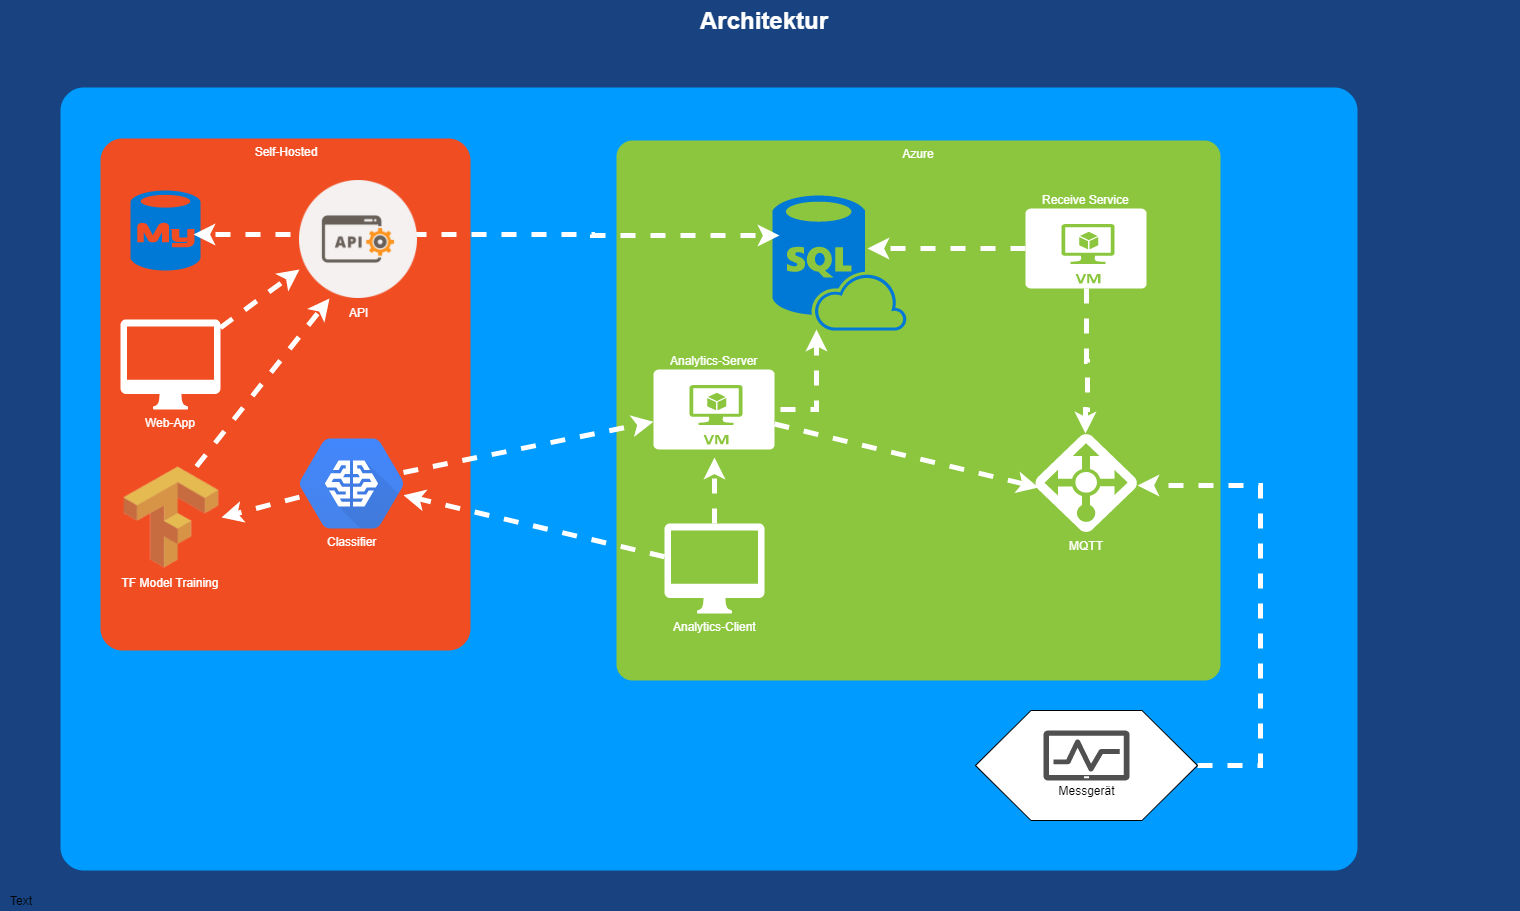
\includegraphics[width=1.0\textwidth]{Architecture}
        \caption{Complete Architecture}
        \label{fig:Architecture}
    \end{figure}

    \subsection{Klassifikation der Messdaten}
        
        Durch die oben beschriebene Messung der Daten sind die physikalischen Werte zu bestimmten sekündlichen Zeitpunkten bestimmt worden.
        Zusätzlich wird nun zur Identifikation der Geräte sowie zum Maschinellen Lernen, genau definierte Zeiträume benötigt in denen bestimmte Geräte aktiv waren.
        Dies bedeutet, dass jedem Zeitpunkt ein oder mehrere Geräte zugewiesen werden. Die einem Gerät zugewiesense Daten werden im weiteren Verlauf gelabelte Daten genannt.\\
        \newline
        Um diese gelabelten Daten zu erheben gibt es verschiedene Möglichkeiten.
        Die Daten können entweder durch eine Person, welche Zeiten zu denen sicher Geräte aktiv waren manuell erfasst werden, oder durch eine Maschine automatisch erhoben werden.
        Zur automatischen Erhebung wird ein Messgerät benötigt, welches zwischen dem zu messenden Gerät und dem Stromnetz zwischengeschalten wird und sobald Strom fließt Daten an den Service übermittelt.
        Die automatisierte Methode ermöglichst es präzisere Zeiten als auch mehr Zeiten und Haushaltsgeräte gleichzeitig zu erfassen.

        Da jedoch für die automatisierte Methode ein weiteres Gerät benötigt wird, werden die Daten manuell durch eine Person erfasst.\\
        \newline
        Für die manuelle Datenerfassung wurde eine progressiv Web-App(vgl. Abbildung \ref{fig:WebApp1}) mit einer einfachen MySQL-Datenbank im Backend erstellt, mit der die Daten sehr einfach erfasst und abgespeichert werden können.

        \begin{figure}[h]
            \centering
            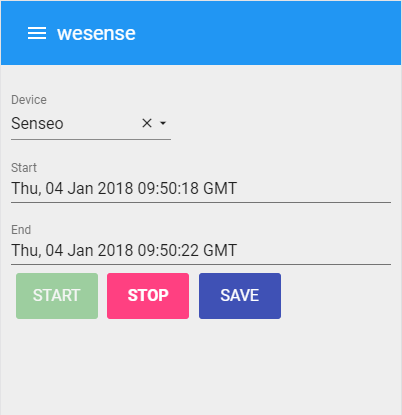
\includegraphics[width=0.5\textwidth]{WesenseConveyWebApp}
            \caption{Screenshot der progressive Web-App}
            \label{fig:WebApp1}
        \end{figure}
    
\section{Visualisierung}\label{VisualisierungWebApp}

        Zusätzlich zur manuellen Erhebung der Daten wurden zur besseren Analyse der Daten verschiedene Visualisierungsmöglichkeiten implementiert.
        Zum einen können die verschiedenen Physikalischen Größen eines Gerätes zu einem bestimmten Zeitpunkt miteinander verglichen werden.
        Hierzu können auch bestimmte Größen zu verschiedenen gelabelten Zeiträumen eines Gerätes verglichen und analysiert werden. 
        Durch diese Visualisierung können sehr gut und genau Gemeinsamkeiten in verschiedenen Größen oder Zeiten erkannt werden.\\
        \newline
        Es werden verschiedene Diagramme sowie Normalisierungen der Daten zur Analyse bereitgestellt.
        Es besteht die Möglichkeit die Daten in einem Liniendiagramm sekündlich oder in frei wählbaren zusammengefassten Datenpunkten, sogennannten Klassen, anzuzeigen.
        Des weiteren können Histogramme mit verschiedenen Klassen gewählt werden.

        \begin{figure}[h]
            \centering
            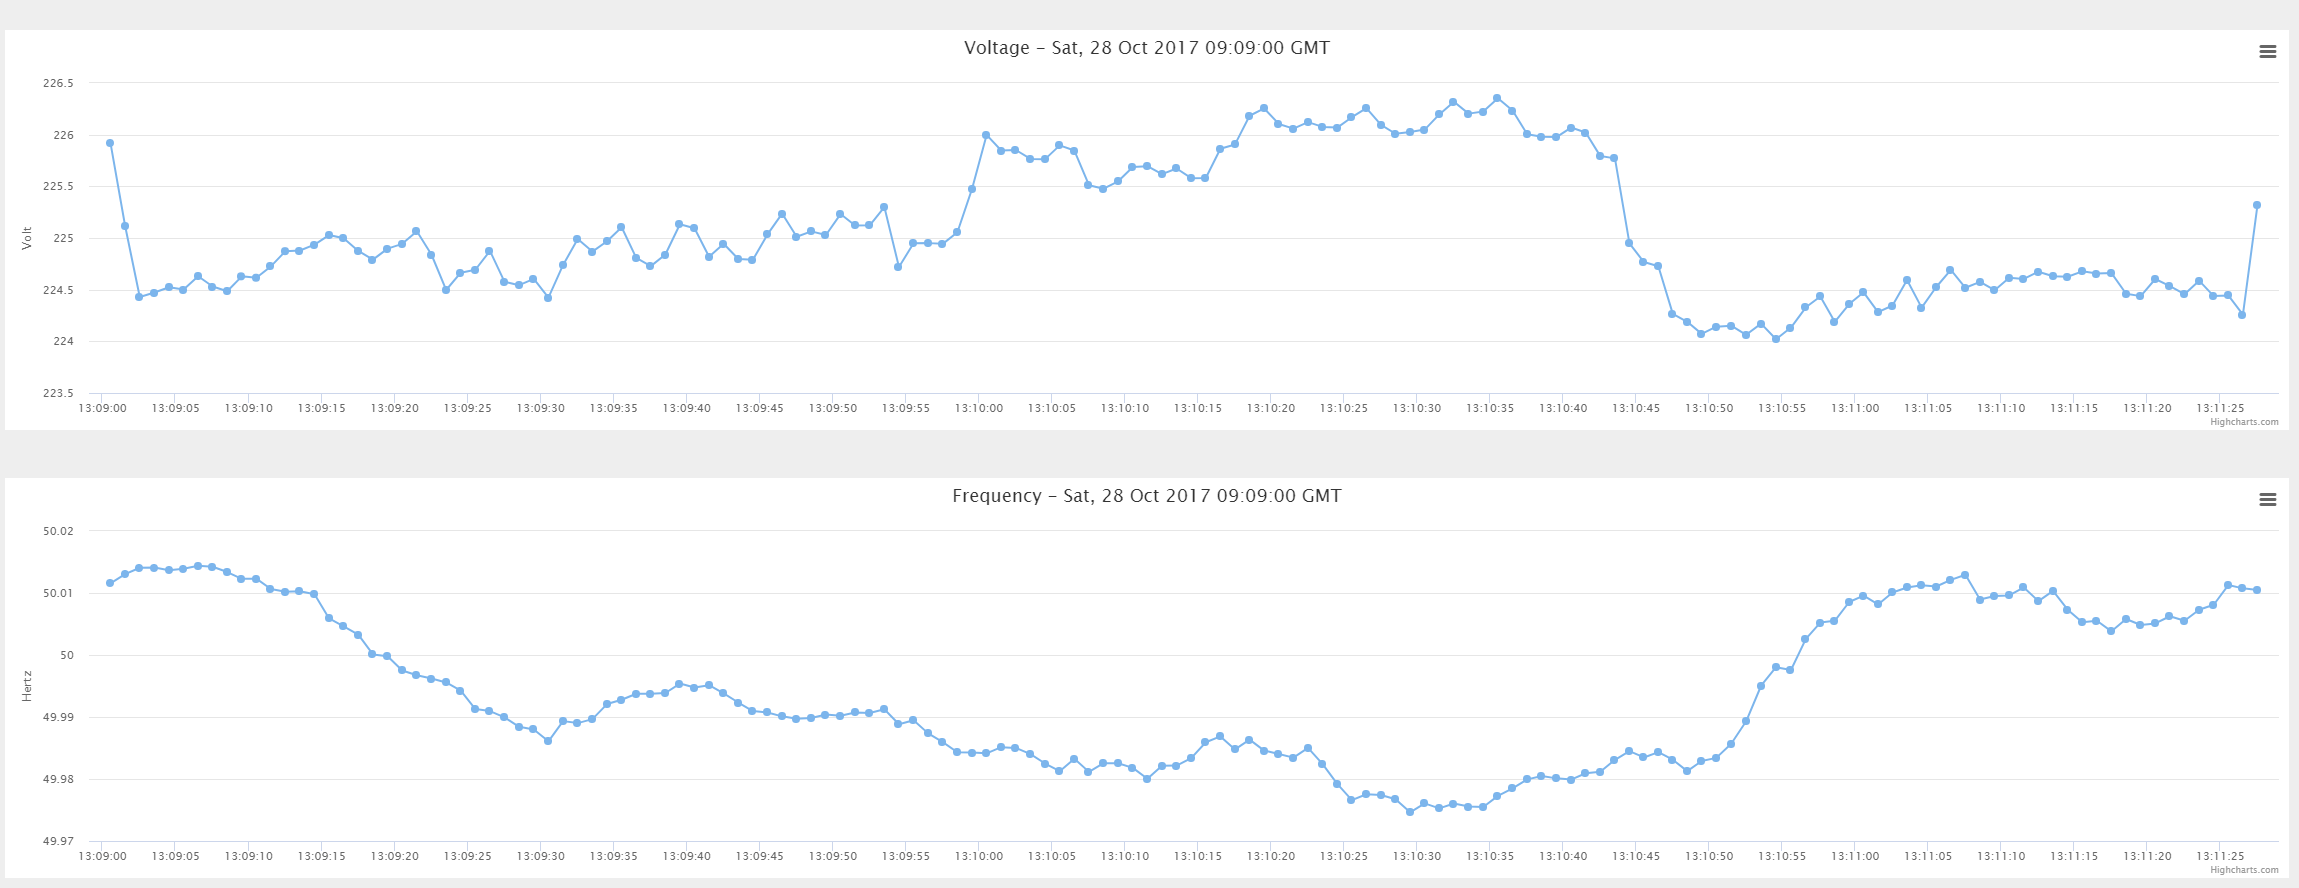
\includegraphics[width=0.75\textwidth]{WesenseConveylineChart}
            \caption{Screenshot eines gelabelten Zeitraumes aus der Web-App}
            \label{fig:WebApp2}
        \end{figure}
        